% !TeX program = xelatex
% Báo cáo môn Kiến trúc phần mềm — Crypto Strategy Lab
% Biên dịch từ thư mục docs/: xelatex main.tex (chạy hai lần)

\documentclass[12pt,a4paper,oneside]{report}

% Ngôn ngữ, font và bố cục
\usepackage[a4paper,top=2.3cm,bottom=2.3cm,left=3cm,right=2.2cm]{geometry}
\usepackage{fontspec}
\usepackage{polyglossia}
\setdefaultlanguage{vietnamese}
\setotherlanguage{english}
\setmainfont{TeX Gyre Termes}
\setsansfont{TeX Gyre Heros}
\setmonofont{Latin Modern Mono}
\usepackage{microtype}
\usepackage{setspace}
\usepackage{enumitem}
\usepackage{titlesec}
\usepackage{fancyhdr}
\usepackage{ragged2e}

% Bảng, hình và màu sắc
\usepackage{graphicx}
\usepackage{float}
\usepackage{caption}
\usepackage{subcaption}
\usepackage{pdflscape}
\usepackage{booktabs}
\usepackage{longtable}
\usepackage{tabularx}
\usepackage{array}
\usepackage{multirow}
\usepackage{makecell}
\usepackage[table]{xcolor}

\definecolor{Primary}{HTML}{155E75}
\definecolor{Secondary}{HTML}{0F766E}
\definecolor{Accent}{HTML}{EA580C}
\definecolor{Success}{HTML}{15803D}
\definecolor{Warning}{HTML}{B45309}
\definecolor{Danger}{HTML}{B91C1C}
\definecolor{Muted}{HTML}{475569}
\definecolor{TableHeader}{HTML}{E2E8F0}
\definecolor{LightPanel}{HTML}{F8FAFC}

\newcolumntype{Y}{>{\RaggedRight\arraybackslash}X}
\newcolumntype{L}[1]{>{\RaggedRight\arraybackslash}p{#1}}
\newcolumntype{C}[1]{>{\Centering\arraybackslash}p{#1}}
\renewcommand{\arraystretch}{1.2}

% Liên kết và tham chiếu
\usepackage{xurl}
\usepackage{hyperref}
\usepackage{bookmark}
\usepackage[capitalise,noabbrev]{cleveref}
\hypersetup{
  unicode=true,
  colorlinks=true,
  linkcolor=Primary,
  citecolor=Secondary,
  urlcolor=Accent,
  pdftitle={Báo cáo Kiến trúc phần mềm — Crypto Strategy Lab},
  pdfauthor={Nhóm 09 — Lớp 23KTPM01},
  pdfsubject={Đồ án cuối kỳ môn Kiến trúc phần mềm},
  pdfkeywords={software architecture, modular monolith, strategy plugin, queue worker, reproducibility}
}
\crefname{chapter}{Chương}{Chương}
\crefname{section}{Mục}{Mục}
\crefname{figure}{Hình}{Hình}
\crefname{table}{Bảng}{Bảng}
\AtBeginDocument{%
  \renewcommand{\chaptername}{Chương}%
  \renewcommand{\contentsname}{Mục lục}%
  \renewcommand{\listfigurename}{Danh mục hình}%
  \renewcommand{\listtablename}{Danh mục bảng}%
  \renewcommand{\figurename}{Hình}%
  \renewcommand{\tablename}{Bảng}%
  \renewcommand{\bibname}{Tài liệu tham khảo}%
}

% Heading, header/footer và tiện ích
\titleformat{\chapter}[display]
  {\normalfont\bfseries\color{Primary}}
  {\filleft\Large\chaptername\ \thechapter}
  {0.5ex}
  {\titlerule\vspace{1ex}\Huge}
\titleformat{\section}{\Large\bfseries\color{Primary}}{\thesection}{0.8em}{}
\titleformat{\subsection}{\large\bfseries\color{Secondary}}{\thesubsection}{0.8em}{}
\titleformat{\subsubsection}{\normalsize\bfseries\color{Muted}}{\thesubsubsection}{0.8em}{}

\pagestyle{fancy}
\fancyhf{}
\fancyhead[L]{\small Crypto Strategy Lab}
\fancyhead[R]{\small\nouppercase{\leftmark}}
\fancyfoot[C]{\thepage}
\renewcommand{\headrulewidth}{0.4pt}
\setlength{\headheight}{15pt}
\setlength{\parindent}{1.1cm}
\setlength{\parskip}{0.25em}
\setlength{\emergencystretch}{3em}
\onehalfspacing
\setlist[itemize]{leftmargin=1.5em,itemsep=0.2em,topsep=0.3em}
\setlist[enumerate]{leftmargin=1.8em,itemsep=0.2em,topsep=0.3em}

\graphicspath{{report-assets/diagrams/}{ui/screens/}{images/}}
\captionsetup{font=small,labelfont=bf,labelsep=period}
\newcommand{\project}{\textit{Crypto Strategy Lab}}
\newcommand{\sourceNote}[1]{\par\vspace{0.2em}{\footnotesize\itshape Nguồn: #1}\par}
\newcommand{\statusVerified}{\textcolor{Success}{\textbf{VERIFIED}}}
\newcommand{\statusPartial}{\textcolor{Warning}{\textbf{PARTIAL}}}
\newcommand{\statusBlocked}{\textcolor{Danger}{\textbf{BLOCKED}}}
\newcommand{\statusPlanned}{\textcolor{Muted}{\textbf{PLANNED}}}
\newcommand{\statusNoClaim}{\textcolor{Muted}{\textbf{NO CLAIM}}}
\newcommand{\archfigure}[4][0.98\linewidth]{%
  \begin{figure}[H]
    \centering
    \includegraphics[width=#1,height=0.72\textheight,keepaspectratio]{#2}
    \caption{#3}
    \label{#4}
    \sourceNote{Nhóm tác giả, tổng hợp từ tài liệu kiến trúc trong repository.}
  \end{figure}
}

\begin{document}

% Trang bìa
\hypersetup{pageanchor=false}
\begin{titlepage}
  \centering
  {\bfseries\Large TRƯỜNG ĐẠI HỌC KHOA HỌC TỰ NHIÊN -- ĐHQG-HCM\par}
  \vspace{0.2cm}
  {\bfseries\large KHOA CÔNG NGHỆ THÔNG TIN\par}
  \vspace{0.8cm}
  \IfFileExists{images/logo.png}{%
    \includegraphics[width=4.2cm]{images/logo.png}
  }{%
    \fcolorbox{Primary}{LightPanel}{%
      \parbox[c][2.7cm][c]{4.8cm}{\centering\bfseries\color{Primary}
      CRYPTO\\STRATEGY LAB}%
    }
  }
  \vspace{0.8cm}
  {\color{Primary}\rule{\textwidth}{1.1pt}\par}
  \vspace{0.65cm}
  {\bfseries\fontsize{25pt}{30pt}\selectfont BÁO CÁO ĐỒ ÁN CUỐI KỲ\par}
  \vspace{0.45cm}
  {\bfseries\Large MÔN KIẾN TRÚC PHẦN MỀM\par}
  \vspace{0.8cm}
  {\bfseries\fontsize{22pt}{27pt}\selectfont\color{Primary} CRYPTO STRATEGY LAB\par}
  \vspace{0.25cm}
  {\large Nền tảng phân tích, kết hợp và đánh giá chiến lược giao dịch Crypto\par}
  \vspace{0.65cm}
  {\color{Primary}\rule{\textwidth}{1.1pt}\par}
  \vspace{0.8cm}
  \begin{tabular}{L{4.1cm}L{9.5cm}}
    \textbf{Nhóm -- Lớp:} & Nhóm 09 -- CSC13106 -- 23KTPM01 \\
    \textbf{Giảng viên:} & PGS.TS. Trần Minh Triết \\
                         & ThS. Trần Văn Quý \\
                         & ThS. Nguyễn Huy Khánh \\
                         & ThS. Ngô Ngọc Đăng Khoa \\
  \end{tabular}
  \vspace{0.65cm}
  \begin{tabular}{C{1.1cm}L{3.1cm}L{7.4cm}}
    \rowcolor{TableHeader}
    \textbf{STT} & \textbf{MSSV} & \textbf{Họ và tên} \\
    1 & 23127221 & Nguyễn Tiến Luật \\
    2 & 23127228 & Phạm Văn Minh \\
    3 & 23127281 & Đặng Nghi Văn \\
    4 & 23127494 & Nguyễn Huỳnh Tiến \\
  \end{tabular}
  \vfill
  {\large Thành phố Hồ Chí Minh, tháng 9 năm 2026\par}
\end{titlepage}
\hypersetup{pageanchor=true}

% Front matter
\pagenumbering{roman}
\setcounter{page}{1}
\chapter*{Tóm tắt}
\addcontentsline{toc}{chapter}{Tóm tắt}

\project{} là nền tảng phục vụ nghiên cứu và thử nghiệm chiến lược giao dịch crypto. Hệ thống tiếp nhận dữ liệu thị trường lịch sử và thời gian thực, cho phép người dùng cấu hình strategy đơn hoặc composite strategy, thực hiện backtest, đánh giá bằng các chỉ số định lượng, duy trì bảng xếp hạng Top-K và bổ sung tín hiệu sentiment từ tin tức. Trọng tâm của đồ án không phải tìm ra chiến lược đầu tư sinh lời, mà là xây dựng một kiến trúc có thể thay đổi, mở rộng, phục hồi và kiểm chứng được theo yêu cầu môn học \cite{de-bai,slide-kien-truc}.

Báo cáo trình bày kiến trúc theo mạch từ architectural drivers đến bằng chứng. Backend được tổ chức theo Modular Monolith với các capability module có public boundary rõ ràng; API và Worker được tách thành hai runtime; Sentiment Service chạy độc lập bằng Python/FastAPI. Các boundary biến thiên được bảo vệ bởi Market Data Provider Adapter, Strategy Plugin/Registry và Strategy Generator contract. Những tác vụ dài sử dụng Queue--Worker, Redis Streams, Transactional Outbox, at-least-once delivery và idempotency. PostgreSQL giữ nguồn dữ liệu nghiệp vụ chuẩn, trong khi Redis đảm nhiệm transport, cache và trạng thái tạm có thể phục hồi \cite{fowler2002,postgresql-docs,redis-streams}.

Phần đánh giá sử dụng quality attribute scenario và ATAM-lite để xem xét modifiability, replaceability, scalability, performance, realtime, reliability, observability và reproducibility. Báo cáo phân biệt rõ kết quả đã kiểm chứng, kết quả kiểm thử có điều khiển, phần còn thiếu bằng chứng LIVE và nội dung mới là kế hoạch. Các con số benchmark được trình bày cùng môi trường và giới hạn đo, không được diễn giải thành SLA production.

\noindent\textbf{Từ khóa:} Software Architecture, Modular Monolith, C4 Model, Strategy Plugin, Queue--Worker, Transactional Outbox, Redis Streams, Reproducibility, ATAM.

\clearpage
\tableofcontents
\clearpage
\addcontentsline{toc}{chapter}{Danh mục hình}
\listoffigures
\clearpage
\addcontentsline{toc}{chapter}{Danh mục bảng}
\listoftables
\clearpage

\chapter*{Thuật ngữ và chữ viết tắt}
\addcontentsline{toc}{chapter}{Thuật ngữ và chữ viết tắt}
\begin{longtable}{L{2.4cm}L{4.5cm}L{7.5cm}}
  \toprule
  \rowcolor{TableHeader}
  \textbf{Ký hiệu} & \textbf{Tên đầy đủ} & \textbf{Ý nghĩa trong báo cáo} \\
  \midrule
  \endfirsthead
  \toprule
  \rowcolor{TableHeader}
  \textbf{Ký hiệu} & \textbf{Tên đầy đủ} & \textbf{Ý nghĩa trong báo cáo} \\
  \midrule
  \endhead
  ADR & Architecture Decision Record & Bản ghi quyết định kiến trúc, phương án thay thế và hệ quả. \\
  ASR & Architecturally Significant Requirement & Yêu cầu có ảnh hưởng trực tiếp đến cấu trúc hệ thống. \\
  ATAM & Architecture Tradeoff Analysis Method & Phương pháp đánh giá kiến trúc bằng scenario và trade-off. \\
  C4 & Context, Container, Component, Code & Bộ view kiến trúc theo nhiều mức phóng đại. \\
  CQRS & Command Query Responsibility Segregation & Tách mô hình ghi và đọc; dự án không triển khai CQRS đầy đủ. \\
  DLQ & Dead Letter Queue & Nơi giữ message thất bại sau khi hết retry budget. \\
  JWT & JSON Web Token & Access token dùng tại public API boundary. \\
  MDD & Maximum Drawdown & Mức sụt giảm lớn nhất trong quá trình backtest. \\
  MVP & Minimum Viable Product & Phạm vi sản phẩm tối thiểu cần chứng minh. \\
  SLA & Service Level Agreement & Cam kết mức dịch vụ; các target demo trong báo cáo không phải SLA. \\
  WSS & WebSocket Secure & Kênh WebSocket qua TLS cho môi trường triển khai. \\
  \bottomrule
\end{longtable}

\clearpage
\pagenumbering{arabic}
\setcounter{page}{1}

% Chương 1
\chapter{Giới thiệu và bối cảnh bài toán}
\label{chap:introduction}

\section{Bối cảnh}

Thị trường cryptocurrency hoạt động liên tục và phát sinh khối lượng dữ liệu lớn theo nhiều cặp giao dịch, timeframe và nguồn thông tin. Một cây nến chuẩn biểu diễn giá mở cửa, cao nhất, thấp nhất, đóng cửa và khối lượng trong một khoảng thời gian. Trader thường phân tích chuỗi nến bằng Moving Average, RSI, Bollinger Bands, Support/Resistance và nhiều phương pháp khác. Tuy nhiên, một strategy đơn lẻ thường chỉ phù hợp với một số market regime nhất định: chiến lược bám xu hướng dễ nhiễu khi thị trường đi ngang, trong khi chiến lược quá mua/quá bán có thể phát tín hiệu sớm trong một xu hướng mạnh.

Đề bài đặt câu hỏi rộng hơn việc cài đặt một indicator: liệu có thể tạo một nền tảng cho phép bổ sung strategy mới, kết hợp chúng, chạy backtest có kiểm soát, đánh giá và liên tục tìm candidate tốt hơn mà không phải viết lại toàn hệ thống hay không \cite{de-bai}. Vì vậy, đối tượng được thiết kế là một \emph{experiment platform}, không phải một trading bot đặt lệnh thật.

\section{Vấn đề kiến trúc}

Một hiện thực ban đầu có thể gom việc gọi Binance, tính indicator, crawl tin tức, inference sentiment, backtest, xếp hạng, lưu database và gửi WebSocket vào một ``God Service''. Cách làm đó có thể chạy được ở quy mô demo nhỏ nhưng tạo nhiều lý do thay đổi trong cùng một component. Khi yêu cầu thêm MACD, thay Binance bằng provider khác, đổi Random Search hoặc tăng số backtest, tác động sẽ lan sang các phần không liên quan.

Theo cách trình bày của seminar, báo cáo không bắt đầu bằng việc lựa chọn Kafka, Kubernetes hay microservices. Chuỗi lập luận được sử dụng là:
\begin{center}
\textbf{Business goal} $\rightarrow$ \textbf{ASR} $\rightarrow$ \textbf{Quality scenario}
$\rightarrow$ \textbf{Decision/tactic} $\rightarrow$ \textbf{Technology} $\rightarrow$ \textbf{Evidence}.
\end{center}
Mỗi công nghệ vì vậy phải trả lời được hai câu hỏi: nó giải quyết driver nào, và bằng chứng nào cho thấy quyết định có hiệu lực.

\section{Mục tiêu và stakeholder}

Các nhóm liên quan và mối quan tâm dùng để dẫn xuất architectural drivers được tổng hợp trong \cref{tab:stakeholders}.

\begin{table}[H]
  \centering
  \caption{Stakeholder và mối quan tâm chính}
  \label{tab:stakeholders}
  \begin{tabularx}{\textwidth}{L{3.2cm}YY}
    \toprule
    \rowcolor{TableHeader}
    \textbf{Stakeholder} & \textbf{Mục tiêu} & \textbf{Mối quan tâm kiến trúc} \\
    \midrule
    User/Trader & Theo dõi market, cấu hình strategy, chạy experiment và xem kết quả. & UI phản hồi, dữ liệu nhất quán, trạng thái rõ, kết quả truy vết được. \\
    Nhóm phát triển & Thêm capability và sửa lỗi trong thời gian đồ án ngắn. & Boundary rõ, test tự động, thay đổi cục bộ, build có kiểm soát. \\
    Team/Operator & Khởi động, demo và chẩn đoán hệ thống. & Health/readiness, log correlation, queue/job state, recovery. \\
    Giảng viên/Reviewer & Kiểm tra chất lượng kiến trúc thay vì chỉ xem tính năng. & C4 nhất quán với code, trade-off hợp lý, scenario và evidence tái kiểm tra được. \\
    External providers & Cung cấp market data và news. & Rate limit, timeout, schema drift, disconnect và payload không tin cậy. \\
    \bottomrule
  \end{tabularx}
\end{table}

\section{Phạm vi và giới hạn}

Phạm vi MVP gồm dữ liệu lịch sử và realtime từ Binance qua adapter; tối đa bốn chart độc lập; bốn strategy cơ sở; composite strategy; backtest; bốn metric bắt buộc; Random Search với stop condition; Queue--Worker; Top-K Leaderboard; news collection; sentiment analysis; và provenance cho Experiment. Bảng \ref{tab:scope} phân biệt rõ phần trong và ngoài phạm vi.

\begin{table}[H]
  \centering
  \caption{Phạm vi và non-goals của đồ án}
  \label{tab:scope}
  \begin{tabularx}{\textwidth}{YY}
    \toprule
    \rowcolor{TableHeader}
    \textbf{Trong phạm vi} & \textbf{Ngoài phạm vi/không tuyên bố} \\
    \midrule
    Nghiên cứu và so sánh strategy trên dữ liệu lịch sử. & Giao dịch tiền thật, quản lý ví, custody hoặc order execution. \\
    Realtime chart và multi-timeframe. & Cam kết dữ liệu provider luôn khả dụng hoặc tuyệt đối chính xác. \\
    Plugin/Registry, composite và replaceable generator. & Upload và chạy plugin không tin cậy ở runtime. \\
    Async jobs, retry, recovery và Top-K projection. & Exactly-once delivery hoặc zero-downtime production SLA. \\
    News/Sentiment qua service boundary có version. & Khuyến nghị đầu tư hoặc cam kết lợi nhuận. \\
    Docker cho Sentiment và local infrastructure. & Kubernetes, Kafka, service mesh hoặc microservice cho mọi module. \\
    \bottomrule
  \end{tabularx}
\end{table}

\section{Đối chiếu yêu cầu chức năng}

Repository hiện có source code và automated test cho các capability chính. Tuy nhiên, mức hiện thực và mức bằng chứng demo LIVE là hai khái niệm khác nhau. Bảng \ref{tab:function-status} dùng trạng thái implementation ở cấp repository; kết quả kiểm chứng chi tiết được trình bày tại \cref{chap:evaluation}.

\begin{longtable}{L{3.2cm}L{2.7cm}L{8.4cm}}
  \caption{Tình trạng các capability chính}\label{tab:function-status}\\
  \toprule
  \rowcolor{TableHeader}
  \textbf{Capability} & \textbf{Tình trạng code} & \textbf{Dấu vết trong repository} \\
  \midrule
  \endfirsthead
  \toprule
  \rowcolor{TableHeader}
  \textbf{Capability} & \textbf{Tình trạng code} & \textbf{Dấu vết trong repository} \\
  \midrule
  \endhead
  Market Data & Implemented & Binance REST/WebSocket adapter, canonical Candle, fixture provider, retry và reconnect. \\
  Multi-timeframe UI & Implemented & Bốn panel giữ pair/timeframe và subscription state độc lập. \\
  Strategy Engine & Implemented & Strategy contract, descriptor, parameter schema, Plugin/Registry. \\
  Strategy Library & Implemented & MA Crossover, RSI, Bollinger Bands và Support/Resistance. \\
  Composite Strategy & Implemented & Majority Vote, Weighted Vote và versioned composite definition. \\
  Search & Implemented & Random Search, deterministic seed/state, finite stop condition và bounded Search Space. \\
  Backtest/Evaluation & Implemented & Historical simulation, Trade/Result bất biến và bốn metric bắt buộc. \\
  Leaderboard & Implemented & Top-K projection, deterministic tie-break và revision. \\
  Reliable Worker & Implemented & Redis Streams, Consumer Group, Outbox, retry, reclaim, idempotency và DLQ. \\
  News/Sentiment & Implemented & RSS normalization, deduplication, analysis lifecycle và FastAPI model runtime. \\
  Public API/Web & Implemented & REST, JWT authorization, WebSocket ticket, reconciliation và các route chính. \\
  Full LIVE demo & Chưa xác minh đầy đủ & Controlled gates có evidence; authenticated LIVE journey và video vẫn còn thiếu. \\
  \bottomrule
\end{longtable}

% Chương 2
\chapter{Architectural Drivers và Quality Attribute Scenarios}
\label{chap:drivers}

\section{Từ yêu cầu chức năng đến ASR}

Không phải mọi yêu cầu đều ảnh hưởng kiến trúc ở cùng mức. Màu sắc của nút bấm thường là quyết định presentation cục bộ; ngược lại, yêu cầu ``News Service lỗi nhưng Market Chart vẫn chạy'' buộc hệ thống có failure boundary. Tương tự, yêu cầu tăng từ hàng trăm lên nhiều nghìn candidate tác động đến execution model, queue, persistence và observability. Đây là các ASR cần được ưu tiên trước khi chọn technology stack \cite{bass2021,cervantes2016}.

\section{Tám driver trọng yếu}

\Cref{tab:drivers} liên kết từng quality attribute với câu hỏi kiểm chứng và tác động trực tiếp lên cấu trúc hệ thống.

\begin{table}[H]
  \centering
  \caption{Architectural drivers của Crypto Strategy Lab}
  \label{tab:drivers}
  \small
  \begin{tabularx}{\textwidth}{L{3.1cm}YL{5.2cm}}
    \toprule
    \rowcolor{TableHeader}
    \textbf{Driver} & \textbf{Câu hỏi} & \textbf{Tác động cấu trúc} \\
    \midrule
    Modifiability & Thêm MACD phải sửa bao nhiêu nơi? & Strategy contract, Plugin/Registry, module boundary. \\
    Replaceability & Đổi generator/provider/model có làm downstream đổi? & Port/adapter, registry và versioned contract. \\
    Scalability & Tăng candidate có thể tăng Worker không? & Queue, Consumer Group, bounded concurrency và DB plan. \\
    Performance & Search dài có giữ HTTP request? & Async acceptance, batching, backpressure và projection. \\
    Realtime & Candle mới đến bốn chart thế nào? & Multiplex WebSocket, coalescing, snapshot và reconciliation. \\
    Reliability & Disconnect/crash được phục hồi ra sao? & Retry, reclaim, Outbox, idempotency và degraded state. \\
    Observability & Có biết job nào lỗi và backlog bao nhiêu? & Correlation identity, progress, log và health endpoint. \\
    Reproducibility & Top-K dùng dữ liệu và strategy version nào? & Frozen Manifest, checksum, fingerprint và immutable Result. \\
    \bottomrule
  \end{tabularx}
\end{table}

\section{Mẫu quality attribute scenario}

Nhóm sử dụng cấu trúc Source--Stimulus--Environment--Artifact--Response--Measure (S--S--E--A--R--M). Measure phải kiểm tra được và được hiểu là target của môi trường demo, không phải production SLA.
Các scenario ưu tiên và measure tương ứng được trình bày tại \cref{tab:quality-scenarios}.

\begin{table}[H]
  \centering
  \caption{Các quality attribute scenario ưu tiên}
  \label{tab:quality-scenarios}
  \scriptsize
  \begin{tabularx}{\textwidth}{L{1.1cm}L{2.6cm}YYY}
    \toprule
    \rowcolor{TableHeader}
    \textbf{ID} & \textbf{Attribute} & \textbf{Stimulus/Artifact} & \textbf{Response} & \textbf{Measure mục tiêu} \\
    \midrule
    QA-01 & Modifiability & Thêm MACD vào Strategy capability. & Thêm plugin, descriptor và test qua Registry. & Không sửa Backtester, Evaluator, Leaderboard hoặc UI business logic. \\
    QA-02 & Replaceability & Thêm generator bên cạnh Random Search. & Resolve theo ID/version và trả Candidate Definition chuẩn. & Queue contract và downstream không đổi. \\
    QA-03 & Modifiability & Chọn Fixture/OKX thay Binance. & Adapter normalize payload/error sang canonical model. & Public API và frontend không đổi. \\
    QA-04 & Reliability & Binance WebSocket disconnect. & Báo reconnecting, backoff, backfill, sort và deduplicate. & Không thiếu/trùng closed Candle trong gap; target demo phục hồi $\leq 30$s. \\
    QA-05 & Scalability & Tăng Worker từ 1 lên 3. & Consumer Group phân phối job; reclaim và dedup. & Target $\geq 2\times$ baseline, không duplicate Result. \\
    QA-06 & Fault isolation & Sentiment process timeout/down. & Retry giới hạn, circuit breaker và degraded state. & Market và technical Backtest tiếp tục; target báo degraded $\leq 5$s. \\
    QA-07 & Reproducibility & Reproduce một Top-K result. & Validate version/checksum và tạo reproduction run mới. & Trade sequence, metrics và fingerprint khớp; không overwrite bản gốc. \\
    QA-08 & Observability & Candidate queue/retry/fail/new best. & Persist progress và phát revision/status. & Trace được bằng correlationId, experimentId, candidateId và jobId. \\
    \bottomrule
  \end{tabularx}
\end{table}

\section{Constraints và giả định}

Nhóm có bốn thành viên và thời gian đồ án giới hạn, do đó chi phí vận hành là constraint quan trọng. Binance, News Provider và Supabase là external dependencies không kiểm soát được availability. Hệ thống không đặt lệnh giao dịch và chỉ xử lý dữ liệu public cho mục đích nghiên cứu. Những scenario cần nhiều host, production traffic hoặc authenticated LIVE session được ghi nhận như khoảng trống kiểm chứng thay vì suy diễn từ unit test.

% Chương 3
\chapter{Kiến trúc tổng thể và các view}
\label{chap:views}

\section{Cách tổ chức tài liệu kiến trúc}

Một view kiến trúc phải trả lời một câu hỏi cụ thể. System Context cho biết hệ thống giao tiếp với ai; Container cho biết các runtime và data store; Component/Module cho biết trách nhiệm và dependency direction; Dynamic View mô tả tương tác theo thời gian. Cách tách view tránh việc nhồi framework, database và module vào cùng một hình \cite{clements2010,brownC4}. Việc nhóm khái niệm theo capability và giữ ngôn ngữ nhất quán giữa các boundary cũng dựa trên tư duy Domain-Driven Design \cite{evans2003}.

\section{C4 Level 1 — System Context}

\archfigure{system-context.pdf}{C4 System Context của Crypto Strategy Lab}{fig:system-context}

Boundary của hệ thống bao gồm Web Dashboard, public API/WebSocket, các capability nghiệp vụ, Worker, persistence và Sentiment runtime. Binance và News Providers nằm ngoài boundary; payload từ các nguồn này được xem là không tin cậy và phải qua adapter. User không truy cập trực tiếp Binance, business tables hoặc Sentiment Service.

\section{C4 Level 2 — Container}

\archfigure[0.94\linewidth]{container-view.pdf}{C4 Container View và các kênh giao tiếp}{fig:container-view}

Vai trò, interface và hướng scale của từng container được đối chiếu trong \cref{tab:containers}.

\begin{table}[H]
  \centering
  \caption{Container catalog}
  \label{tab:containers}
  \small
  \begin{tabularx}{\textwidth}{L{2.6cm}YYL{3.2cm}}
    \toprule
    \rowcolor{TableHeader}
    \textbf{Container} & \textbf{Trách nhiệm} & \textbf{Interface} & \textbf{Scale strategy} \\
    \midrule
    apps/web & UI, chart, subscription state, progress và result view. & REST, WebSocket, Supabase Auth. & Web replica/CDN khi cần. \\
    apps/api & Public contract, validation, WebSocket gateway và command orchestration. & HTTP/JSON, WebSocket, JDBC. & Scale sau khi kiểm chứng state strategy. \\
    apps/worker & Search coordination, Backtest/Evaluation, Ranking và News jobs. & Redis Streams, JDBC, internal HTTP. & Tăng instance trong Consumer Group. \\
    apps/sentiment & Stateless text inference có model provenance. & Internal HTTP/JSON, health/readiness. & Nhiều instance độc lập nếu inference là bottleneck. \\
    PostgreSQL & Business source of truth và Outbox. & JDBC/PostgreSQL. & Pool/query/index plan là giới hạn chính. \\
    Redis & Streams, pending delivery, cache và progress tạm. & Redis protocol. & Điều chỉnh topology theo measurement. \\
    \bottomrule
  \end{tabularx}
\end{table}

\section{C4 Level 3 — Backend Module View}

\archfigure[0.96\linewidth]{module-view.pdf}{Dependency direction giữa các module backend}{fig:module-view}

Backend Java có hai composition root là API và Worker. Business capability chỉ công khai kiểu và port ổn định trong package \texttt{api}; implementation nằm trong \texttt{internal}. Persistence triển khai output port của capability owner, không trở thành nơi chứa business policy. Các rule này được kiểm tra bằng Gradle module graph và ArchUnit, bao gồm quy tắc không import chéo implementation, không tạo cycle và giữ Strategy contract độc lập Spring/JDBC.
Ranh giới trách nhiệm và các hành vi bị cấm ở mỗi module được tóm tắt tại \cref{tab:module-responsibilities}.

\begin{longtable}{L{3.2cm}L{5.1cm}L{6cm}}
  \caption{Bounded Context và module trách nhiệm}\label{tab:module-responsibilities}\\
  \toprule
  \rowcolor{TableHeader}
  \textbf{Context/module} & \textbf{Trách nhiệm} & \textbf{Không được làm} \\
  \midrule
  \endfirsthead
  \toprule
  \rowcolor{TableHeader}
  \textbf{Context/module} & \textbf{Trách nhiệm} & \textbf{Không được làm} \\
  \midrule
  \endhead
  market-data & Canonical Candle, provider port, Binance/fixture adapter và recovery. & Để provider model thoát ra public contract. \\
  strategy-core & Strategy, Signal, descriptor, schema và Registry. & Gọi network, database hoặc phụ thuộc Spring. \\
  strategies & MA, RSI, Bollinger, Support/Resistance plugin. & Điều phối Search hoặc Backtest. \\
  combination & Composite factory, Majority/Weighted policy. & Tính metrics hoặc Ranking. \\
  experiment & Manifest, lifecycle, version và reproduction identity. & Chứa Strategy/Backtest algorithm. \\
  search & Generator Registry, candidate proposal và stop condition. & Chạy Backtest hoặc cập nhật Top-K. \\
  experiment-execution & Điều phối xuyên capability và durable decision. & Sở hữu thuật toán capability hoặc truy cập table trực tiếp. \\
  backtesting & Mô phỏng execution, Trade và Result. & Biết generator hoặc Ranking implementation. \\
  evaluation & Tính metric versioned từ Backtest Result. & Tạo Strategy hoặc Top-K. \\
  leaderboard & Score, tie-break, Top-K và revision. & Chạy Search/Backtest. \\
  news & Provider contract, normalize/dedup, sentiment ownership. & Phụ thuộc model Python cụ thể. \\
  persistence & JDBC/Redis adapter cho output port. & Chứa business policy hoặc bị capability import ngược. \\
  \bottomrule
\end{longtable}

\section{Deployment View}

\archfigure[0.9\linewidth]{deployment-view.pdf}{Deployment View cho môi trường local/demo}{fig:deployment-view}

API và Worker là hai JVM process khác nhau dù dùng lại các capability module. Việc tách runtime giúp HTTP/WebSocket không chia cùng failure domain và thread pool với Backtest dài. Sentiment Service được container hóa riêng do dependency ML, startup time và failure mode khác Java. PostgreSQL/Supabase nằm ngoài local Compose trong cấu hình hiện tại; Redis và Sentiment có thể chạy local/container.

\section{Data ownership và mô hình dữ liệu khái niệm}

\archfigure[0.98\linewidth]{conceptual-data-model.pdf}{Mô hình dữ liệu khái niệm và quan hệ provenance}{fig:conceptual-data-model}

\Cref{tab:data-ownership} chỉ rõ capability owner, nguồn dữ liệu chuẩn và invariant tương ứng; đây là cơ sở để tránh shared-database coupling không kiểm soát.

\begin{table}[H]
  \centering
  \caption{Phân quyền sở hữu dữ liệu}
  \label{tab:data-ownership}
  \small
  \begin{tabularx}{\textwidth}{L{3cm}YL{2.5cm}Y}
    \toprule
    \rowcolor{TableHeader}
    \textbf{Capability} & \textbf{Dữ liệu sở hữu} & \textbf{Nguồn chuẩn} & \textbf{Quy tắc} \\
    \midrule
    Market Data & Asset, pair, Candle, Dataset Version. & PostgreSQL & Closed Candle idempotent; Dataset có checksum. \\
    Strategy & Strategy/User Strategy/Composite version. & PostgreSQL & Published version bất biến; descriptor có fingerprint. \\
    Experiment & Manifest, Candidate, Job, Attempt. & PostgreSQL & Manifest đóng băng input; attempt tách khỏi logical job. \\
    Backtest/Evaluation & Result, Trade, metrics. & PostgreSQL & Result thành công bất biến và liên kết Candidate. \\
    Leaderboard & Revision và Entry. & PostgreSQL & Projection có thể rebuild từ Evaluation Result. \\
    News & News Item, analysis lifecycle, Sentiment Result. & PostgreSQL & Dedup bằng source/content identity; model version được lưu. \\
    Platform & Outbox, processed message, idempotency record. & PostgreSQL & Redis mất không làm mất business truth. \\
    \bottomrule
  \end{tabularx}
\end{table}

% Chương 4
\chapter{Các quyết định kiến trúc và trade-off}
\label{chap:decisions}

\section{Modular Monolith thay vì chia nhỏ sớm}

Nhóm chọn Modular Monolith cho backend cốt lõi theo ADR-0001. Quyết định phù hợp với quy mô nhóm, thời gian đồ án và nhu cầu giữ transaction nội bộ đơn giản. Boundary được biểu diễn bằng Gradle subproject, public package và architecture test thay vì chỉ là quy ước. API/Worker có thể reuse capability mà không nhân bản domain model.

Giá phải trả là mọi module vẫn được build và release cùng repository; boundary có thể suy thoái nếu bypass public contract. Nhóm giảm rủi ro bằng dependency matrix, ArchUnit và ADR review. Microservices chỉ được dùng tại Sentiment boundary, nơi có driver thật về runtime/dependency/failure isolation.

\section{API--Worker split}

Public API nhận command, validate, ghi durable state và trả ID sớm. Worker thực thi Search, Backtest, Evaluation và background News/Sentiment. Boundary này ngăn tác vụ CPU dài giữ HTTP request, hỗ trợ retry và cho phép tăng Worker mà không sửa core contract. Đổi lại, người dùng quan sát eventual consistency: trạng thái ban đầu có thể là \texttt{QUEUED}, sau đó mới chuyển sang \texttt{RUNNING}/\texttt{COMPLETED}.

\section{Ports, Adapter và Registry}

Market Data Provider là output port; Binance và Fixture là adapter. Mọi payload được normalize sang canonical Candle trước khi đi vào domain. Nhờ đó, frontend và Strategy không phụ thuộc symbol, interval hay error shape riêng của Binance.

Strategy Plugin cung cấp descriptor, semantic version, parameter schema và hàm phân tích trả BUY/SELL/HOLD. Registry giữ danh sách trusted plugin compile-time. Việc thêm strategy mới tập trung trong module \texttt{strategies} và composition registration, thay vì thêm chuỗi \texttt{if/else} tại Controller, Backtester và UI. Đây là ứng dụng Strategy/Registry/Dependency Injection theo mục tiêu extensibility \cite{gamma1994}.

Strategy Generator cũng được bảo vệ bằng contract. Random Search hiện thực interface chuẩn và sinh Candidate Definition; generator khác có thể được đăng ký theo ID/version. Search không chạy Backtest, còn Backtester không biết candidate được sinh bằng thuật toán nào.

\section{Realtime bằng WebSocket}

REST phù hợp cho snapshot, history và command; WebSocket phát update theo subscription. API multiplex subscription theo pair/timeframe, coalesce intermediate open-Candle update khi outbound chậm và không bỏ closed Candle hoặc completion event. Client giữ event identity/revision để bỏ stale update và gọi REST reconciliation sau reconnect. Trade-off là lifecycle, reconnect và ordering phức tạp hơn polling đơn giản.

\section{Queue--Worker và Transactional Outbox}

Một command tạo Experiment cần ghi Manifest, Job và ý định publish trong cùng database transaction. Nếu ghi database thành công nhưng publish Redis thất bại, Outbox Publisher có thể thử lại. Nếu publish thành công nhiều lần, consumer dùng stable message/job identity và durable processed record để ngăn business effect trùng. Mô hình này chấp nhận at-least-once delivery thay vì tuyên bố exactly-once \cite{richardson2019,kleppmann2017}.

ACK chỉ được gửi sau durable commit. Worker crash trước ACK để message ở pending list; consumer khác có thể reclaim sau idle boundary. Lỗi transient dùng bounded retry/backoff; lỗi hết budget được đưa vào DLQ và trạng thái failure được lưu có cấu trúc. Redis cung cấp transport nhanh nhưng không giữ bản duy nhất của Manifest, Job, Result hoặc Leaderboard.

\section{Sentiment Service boundary}

Python/FastAPI được tách vì TensorFlow/Keras có dependency, lifecycle và resource profile khác Java. Service nhận text đã normalize, không tự crawl URL và không truy cập shared database. Contract trả label, confidence, polarity score và model/preprocessing version. Worker chịu timeout, retry, circuit breaker và persist lifecycle; failure của Sentiment không được lan sang Market hoặc technical Backtest.

\section{Frozen provenance và reproducibility}

Experiment Manifest đóng băng Dataset version/checksum, Strategy reference/version/parameters, Backtest assumptions, Search config, metric/ranking version, software version và git commit. Candidate, Result, Trade và Evaluation Result giữ quan hệ bất biến với Manifest. Reproduction tạo một run mới và so sánh fingerprint/trade/metrics; không overwrite kết quả gốc. Cơ chế này biến một dòng Leaderboard từ ``con số hiện tại'' thành một bằng chứng có nguồn gốc.

\section{Ma trận quyết định và trade-off}

\Cref{tab:tradeoffs} đặt mỗi quyết định cạnh driver, lợi ích và chi phí để công nghệ không bị trình bày như mục tiêu tự thân.

\begin{longtable}{L{3cm}L{2.5cm}L{4cm}L{4cm}}
  \caption{Decision--driver--trade-off matrix}\label{tab:tradeoffs}\\
  \toprule
  \rowcolor{TableHeader}
  \textbf{Quyết định} & \textbf{Driver} & \textbf{Lợi ích} & \textbf{Giá phải trả/rủi ro} \\
  \midrule
  \endfirsthead
  \toprule
  \rowcolor{TableHeader}
  \textbf{Quyết định} & \textbf{Driver} & \textbf{Lợi ích} & \textbf{Giá phải trả/rủi ro} \\
  \midrule
  \endhead
  Modular Monolith & Modifiability & Phát triển/deploy đơn giản, transaction nội bộ. & Cần test để boundary không suy thoái. \\
  API/Worker split & Performance, isolation & HTTP phản hồi nhanh; scale compute riêng. & Eventual consistency, thêm process vận hành. \\
  Plugin/Registry & Extensibility & Thêm Strategy cục bộ, catalog tự mô tả. & Quản lý schema, identity và version. \\
  Provider Adapter & Replaceability & Core/frontend độc lập provider payload. & Mapping/error translation và contract test. \\
  WebSocket & Realtime & Push update hiệu quả, subscription linh hoạt. & Reconnect, ordering, backpressure phức tạp. \\
  Redis Streams & Scalability & Consumer Group, pending/reclaim, scale Worker. & Duplicate, queue operation và Redis availability. \\
  Transactional Outbox & Reliability & Không mất ý định publish sau DB commit. & Publisher, cleanup và observability bổ sung. \\
  At-least-once + idempotency & Correctness & Retry/recovery an toàn hơn. & Stable identity và durable dedup state. \\
  Sentiment service riêng & Isolation, replaceability & Tách ML runtime/model lifecycle. & HTTP contract, timeout và container mới. \\
  Frozen Manifest & Reproducibility & Truy vết và tái lập exact input. & Storage/version governance và validation. \\
  Leaderboard projection & Read performance & Query Top-K nhanh, revision rõ. & Reconciliation/rebuild khi projection lệch. \\
  Không full CQRS/Event Sourcing & Simplicity & Giảm độ phức tạp MVP. & Không có generic replay/temporal state toàn hệ thống. \\
  \bottomrule
\end{longtable}

% Chương 5
\chapter{Các luồng runtime trọng yếu}
\label{chap:runtime}

\section{Historical Market Data}

Khi người dùng chọn pair, timeframe và range, Web gửi query chuẩn đến API. Market Data Module kiểm tra cache; cache miss dẫn đến các request phân trang qua Binance Adapter. Adapter xử lý rate limit, timeout và provider error, sau đó module validate, normalize, sắp xếp và deduplicate Candle. Closed Candle và Dataset reference được lưu idempotently; cache chỉ là lớp tăng tốc có TTL/version. Public response luôn dùng canonical contract.

\section{Realtime Candle và phục hồi}

\archfigure[0.98\linewidth]{realtime-recovery.pdf}{Luồng realtime, reconnect và gap recovery}{fig:realtime-recovery}

Một upstream stream có thể được chia sẻ cho nhiều subscriber cùng pair/timeframe. Khi mất kết nối, API không giả trạng thái connected mà phát \texttt{RECONNECTING}. Sau bounded exponential backoff, Market Module backfill từ closed Candle cuối đã xác nhận, hợp nhất vùng dữ liệu overlap và deduplicate theo provider--pair--timeframe--openTime. UI giữ snapshot hiện có, đánh dấu stale/recovering và reconcile sau khi kết nối lại.

\section{Strategy, Backtest và Evaluation}

\archfigure[0.95\linewidth]{strategy-backtest-evaluation.pdf}{Luồng Strategy--Backtest--Evaluation}{fig:strategy-backtest-evaluation}

Worker chỉ bắt đầu khi resolve được Manifest, Dataset checksum và Strategy/Composite version. Registry validate parameters trước khi tạo instance. Backtester đưa ordered Candle vào Strategy, diễn giải BUY/SELL/HOLD theo execution assumptions và tạo ordered Trade sequence. Evaluator tính metric độc lập; trường hợp không có Trade là business result hợp lệ. Nếu version hoặc checksum sai, Job thất bại có cấu trúc và không tạo partial Result.

\section{Search, Queue và Leaderboard}

\begin{landscape}
\archfigure[0.98\linewidth]{search-queue-leaderboard.pdf}{Luồng tạo Experiment, xử lý Candidate và cập nhật Top-K}{fig:search-queue-leaderboard}
\end{landscape}

Điểm quan trọng của luồng là ba transaction boundary: (1) tạo Manifest/Job/Outbox; (2) tạo Candidate/Backtest Job/Outbox cùng durable generator state; (3) commit Result/Evaluation/Outbox trước ACK. Coordinator duy trì bounded in-flight window và stop condition. Ranking xử lý \texttt{CANDIDATE\_EVALUATED} idempotently, tạo Leaderboard revision và phát update hint; frontend luôn có thể tải authoritative snapshot từ REST.

\section{News và Sentiment}

\archfigure[0.98\linewidth]{news-sentiment.pdf}{Luồng News collection và Sentiment Analysis}{fig:news-sentiment}

News Adapter chuyển raw payload thành News Item chuẩn, sanitize nội dung, tạo content hash và loại duplicate. Worker claim analysis lease và gọi versioned Sentiment contract. Response chỉ được persist khi đúng lease đang active và nằm trong range hợp lệ. Lỗi retryable giữ trạng thái minh bạch; UI vẫn đọc được News Item ngay cả khi sentiment tạm unavailable.

\section{Failure isolation}

\archfigure[0.94\linewidth]{failure-isolation.pdf}{Các failure boundary và cơ chế phục hồi}{fig:failure-isolation}

Ba nhánh failure được thiết kế độc lập. Redis/Worker failure dựa trên Outbox, pending reclaim và durable dedup. Sentiment failure chỉ làm degraded News Analysis. WebSocket failure giữ snapshot và dùng reconnect/reconciliation. PostgreSQL failure được xử lý fail-closed cho durable command; hệ thống không dùng Redis để giả một commit nghiệp vụ chưa xảy ra.

\section{Leaderboard provenance}

\archfigure[0.98\linewidth]{leaderboard-provenance.pdf}{Đường truy vết từ Leaderboard đến input bất biến}{fig:leaderboard-provenance}

Một entry được truy qua Evaluation Result, Backtest Result, successful Attempt, Candidate và frozen Manifest. Manifest dẫn đến Dataset checksum, Strategy version/parameters, assumptions, metric/ranking version và software identity. Khi reproduce, hệ thống tạo graph kết quả mới và trả verdict \texttt{MATCHED}/\texttt{MISMATCHED}; kết quả cũ vẫn bất biến.

% Chương 6
\chapter{Hiện thực hệ thống}
\label{chap:implementation}

\section{Technology stack đã xác nhận}

Các phiên bản và capability trong mục này được đối chiếu trực tiếp với build scripts, package manifests, workflow và source code tại repository của nhóm \cite{project-repository}.
Danh sách công nghệ, phiên bản và vai trò đã xác nhận được tổng hợp trong \cref{tab:tech-stack}.

\begin{table}[H]
  \centering
  \caption{Technology stack từ source/configuration}
  \label{tab:tech-stack}
  \small
  \begin{tabularx}{\textwidth}{L{3.2cm}L{4.1cm}Y}
    \toprule
    \rowcolor{TableHeader}
    \textbf{Lớp} & \textbf{Công nghệ} & \textbf{Vai trò} \\
    \midrule
    Backend & Java 21, Spring Boot 3.5.16, Gradle 8.14.5 & API, Worker, capability module và build conventions. \\
    Frontend & Next.js 16.3.4, React 19.1, TypeScript 5.9 & Dashboard, authentication, realtime và feature routes. \\
    Sentiment & Python 3.11--3.12, FastAPI 0.115.12, TensorFlow 2.19 & Versioned inference runtime và health/readiness. \\
    Persistence & PostgreSQL/Supabase, JDBC migrations & Durable business truth, Outbox và projection. \\
    Async/cache & Redis 7, Redis Streams & Queue, Consumer Group, transient cache/progress. \\
    Test & JUnit 5.12, ArchUnit 1.5, Pytest, Vitest, Playwright & Unit, contract, architecture, integration và browser test. \\
    Delivery & Docker, Docker Compose, GitHub Actions & Sentiment image, local runtime và automated quality gates. \\
    \bottomrule
  \end{tabularx}
\end{table}

\section{Strategy Engine và thư viện strategy}

Strategy contract nhận context/candle batch và trả decision chuẩn. Descriptor mô tả plugin ID, semantic version, display name, parameter rules, supported signal và search range hint. Registry từ chối identity trùng. Trusted catalog hiện đăng ký bốn plugin:

\begin{itemize}
  \item \textbf{MA Crossover}: so sánh fast/slow moving average và yêu cầu fast period nhỏ hơn slow period;
  \item \textbf{RSI}: sử dụng period cùng ngưỡng oversold/overbought;
  \item \textbf{Bollinger Bands}: dùng moving window và độ lệch chuẩn để xác định band;
  \item \textbf{Support/Resistance}: nhận diện vùng giá trong lookback window và tolerance.
\end{itemize}

Composite Strategy chứa ordered component snapshots và policy version. Majority Vote chọn tín hiệu chiếm đa số; Weighted Vote nhân signal encoding với trọng số và threshold. Tie hoặc score nằm trong neutral band tạo HOLD. Policy nằm ngoài Strategy implementation để có thể thay quy tắc combine mà không sửa từng plugin.

\section{Search Space và điều phối Experiment}

Random Search dùng seed/state bất biến để có thể tiếp tục và tái tạo candidate sequence. Search Space hỗ trợ strategy pool, parameter range và constraint; composite refill giữ bounded in-flight thay vì đổ toàn bộ candidate vào queue. Stop condition hữu hạn theo maximum candidates và trạng thái terminal. Durable decision/fence ngăn hai Coordinator đồng thời cấp phát cùng một slot sau retry/recovery.

\section{Backtesting assumptions và metrics}

Backtest không giả định một signal chính là giao dịch tức thì. Execution assumptions quy định thời điểm vào/thoát, capital, fee và dữ liệu được phép nhìn thấy nhằm tránh look-ahead bias. Strategy chỉ được đánh giá trên ordered Candle và evaluation time. Result lưu initial/final capital cùng ordered Trade; Evaluation tách khỏi Strategy implementation.
Ý nghĩa và giới hạn diễn giải của từng metric được nêu tại \cref{tab:metrics}.

\begin{table}[H]
  \centering
  \caption{Các metric đánh giá bắt buộc}
  \label{tab:metrics}
  \begin{tabularx}{\textwidth}{L{3.3cm}L{4.3cm}Y}
    \toprule
    \rowcolor{TableHeader}
    \textbf{Metric} & \textbf{Ý nghĩa} & \textbf{Lưu ý diễn giải} \\
    \midrule
    Total Return & Tỷ lệ thay đổi capital sau backtest. & Không đủ để kết luận strategy ổn định. \\
    Win Rate & Tỷ lệ trade có profit dương. & Cần đọc cùng payoff và số lượng trade. \\
    Maximum Drawdown & Sụt giảm lớn nhất từ đỉnh equity đến đáy tiếp theo. & Đại diện rủi ro đường đi, không chỉ kết quả cuối. \\
    Number of Trades & Số giao dịch hoàn tất. & Mẫu quá nhỏ làm metric khó tổng quát. \\
    Overall Score & Hàm xếp hạng có version từ các input metric. & Phải lưu ranking/metric version và deterministic tie-break. \\
    \bottomrule
  \end{tabularx}
\end{table}

\section{Leaderboard và dữ liệu bất biến}

Leaderboard là read projection theo Experiment. Mỗi revision ghi Top-K và ordered Entry; tie-break ổn định để cùng input tạo cùng order. Entry liên kết Evaluation Result thay vì copy một score không nguồn gốc. Khi retry Candidate, unique identity và idempotency ngăn tạo nhiều Result/Entry cho cùng business outcome.

\section{Giao diện người dùng}

Web được chia theo feature boundary cho Market, Strategy, Search/Leaderboard, Backtest Result và News. Authentication/session nằm ở foundation layer; feature chỉ gọi typed API/realtime client. \Cref{fig:ui-market,fig:ui-search,fig:ui-backtest} là tài liệu prototype dùng để minh họa thiết kế giao diện, không được xem là screenshot của phiên LIVE.

\begin{figure}[H]
  \centering
  
\includegraphics[width=0.94\linewidth,height=0.68\textheight,keepaspectratio]{\detokenize{ui/screens/Market Dashboard.png}}
  \caption{UI prototype — Market Dashboard nhiều timeframe}
  \label{fig:ui-market}
  \sourceNote{Tài liệu prototype tại \texttt{docs/ui/screens}; không phải LIVE evidence.}
\end{figure}

\begin{figure}[H]
  \centering
  
\includegraphics[width=0.94\linewidth,height=0.68\textheight,keepaspectratio]{\detokenize{ui/screens/Search & Leaderboard.png}}
  \caption{UI prototype — Search progress và Leaderboard}
  \label{fig:ui-search}
  \sourceNote{Tài liệu prototype tại \texttt{docs/ui/screens}; không phải LIVE evidence.}
\end{figure}

\begin{figure}[H]
  \centering
  
\includegraphics[width=0.94\linewidth,height=0.68\textheight,keepaspectratio]{\detokenize{ui/screens/Backtest Results.png}}
  \caption{UI prototype — Backtest Result và Trade detail}
  \label{fig:ui-backtest}
  \sourceNote{Tài liệu prototype tại \texttt{docs/ui/screens}; không phải LIVE evidence.}
\end{figure}

% Chương 7
\chapter{Reliability, Scalability, Security và Observability}
\label{chap:quality-tactics}

\section{Backpressure và bounded work}

API không đợi Search hoàn tất mà trả resource ID sau durable acceptance. Coordinator cấp phát candidate theo bounded in-flight window; Worker dùng fixed thread pool và semaphore/concurrency configuration. Batching giảm overhead nhưng kích thước batch phải được giữ trong giới hạn memory, DB connection và job timeout. Đây là cách làm backlog hữu hạn và quan sát được thay vì sinh vô hạn task vào Redis.

\section{Scale ngang Worker}

Các Worker dùng cùng stream/group nhưng consumer name riêng. Redis Consumer Group phân phối message; PostgreSQL giữ Job/Attempt/Result. Scale từ một lên nhiều Worker không yêu cầu sửa Strategy, Backtester hay Evaluation contract. Bottleneck có thể chuyển từ CPU sang Redis, database pool, dataset loading hoặc write contention; vì vậy scale-out phải đi cùng measurement queue lag, throughput, duplicate count và DB utilization.

Kịch bản 100.000 backtest không đồng nghĩa đẩy 100.000 message cùng lúc. Kiến trúc dự kiến phân trang/generate theo window, ưu tiên bounded queue, giới hạn concurrency toàn Experiment và có stop/cancel semantics. Nếu workload vượt một host, Worker có thể tăng instance; nếu database trở thành bottleneck, cần tối ưu batch persistence, index, connection budget hoặc partitioning trước khi thêm công nghệ mới.

\section{Retry, recovery và deduplication}

Các failure mode, tactic, invariant và tín hiệu quan sát tương ứng được hệ thống hóa trong \cref{tab:reliability-tactics}.

\begin{table}[H]
  \centering
  \caption{Reliability tactics theo failure mode}
  \label{tab:reliability-tactics}
  \small
  \begin{tabularx}{\textwidth}{L{3.1cm}YYL{3.2cm}}
    \toprule
    \rowcolor{TableHeader}
    \textbf{Failure} & \textbf{Tactic} & \textbf{Invariant} & \textbf{Quan sát} \\
    \midrule
    Publish Redis lỗi & Transactional Outbox và republish. & Intent đã commit không bị mất. & publish attempt, last error. \\
    Worker crash & Pending reclaim/recovery sweep. & Cùng Job có stable identity. & pending age, consumer/attempt. \\
    Duplicate delivery & Durable processed record/idempotent write. & Tối đa một business Result hợp lệ. & duplicate count, message ID. \\
    Lỗi transient & Bounded retry và exponential backoff. & Không retry vô hạn. & attempt no., next retry, error code. \\
    Lỗi permanent & FAILED/DLQ và redacted reason. & Không ACK như thành công. & DLQ depth, failure status. \\
    Redis mất tạm & Rebuild transport/progress từ PostgreSQL/Outbox. & Redis không là business truth. & queue health, recovery lag. \\
    Sentiment down & Timeout, circuit breaker, degraded lifecycle. & Market/technical flow không bị chặn. & circuit state, analysis status. \\
    WebSocket mất & Reconnect, resubscribe, REST reconcile. & Client không dùng stale revision. & connection state, revision. \\
    \bottomrule
  \end{tabularx}
\end{table}

\section{Observability}

Một lỗi background không thể chỉ xuất hiện trong console. Request, Experiment, Candidate, Job, Attempt và message cần correlation identity để truy một flow xuyên API, Outbox, Redis và Worker. Progress snapshot tối thiểu gồm queued/running/completed/failed count, best score, revision và terminal reason. Liveness chỉ cho biết process sống; readiness cho biết runtime có đủ dependency bắt buộc để nhận work.

Các target observability trong tài liệu là khả năng nhìn thấy progress trong vài giây, trace theo identity và phân biệt retryable/permanent failure. Repository có Spring Boot Actuator, structured domain state và WebSocket progress; chưa tuyên bố có production metrics backend hoặc distributed tracing platform hoàn chỉnh.

\section{Security boundary}

Web đăng nhập qua Supabase Auth và gửi JWT đến API. Backend xác thực issuer, JWKS và audience, sau đó kiểm tra ownership theo user cho Strategy, Experiment và Result. WebSocket dùng ticket ngắn hạn thay vì đặt access token dài hạn trong URL. Browser chỉ chứa biến \texttt{NEXT\_PUBLIC}; database password, service-role key và Sentiment token không được phát xuống client.

Sentiment endpoint là internal boundary có service token; Python không tự fetch URL do người dùng cung cấp. External provider payload được validate/sanitize; public error không lộ stack trace hoặc credential. Migrations là forward-only source of truth và secret không được commit vào repository/evidence.

% Chương 8
\chapter{Đánh giá kiến trúc và Architecture Proof}
\label{chap:evaluation}

\section{Phương pháp ATAM-lite}

ATAM-lite được dùng như một ``crash test'' cho kiến trúc: đưa scenario thay đổi hoặc failure vào, xác định sensitivity point, quan sát response và ghi trade-off \cite{bass2021,cervantes2016}. Mục tiêu không phải chấm sơ đồ đẹp mà là chứng minh boundary tồn tại trong code và hành vi.
Kết quả đối chiếu giữa scenario, tactic, measure và evidence được trình bày tại \cref{tab:architecture-proof}.

\begin{longtable}{L{2.6cm}L{2.8cm}L{3.8cm}L{2cm}L{1.8cm}}
  \caption{Architecture proof theo scenario}\label{tab:architecture-proof}\\
  \toprule
  \rowcolor{TableHeader}
  \textbf{Scenario} & \textbf{Decision/tactic} & \textbf{Response và measure} & \textbf{Evidence} & \textbf{Status} \\
  \midrule
  \endfirsthead
  \toprule
  \rowcolor{TableHeader}
  \textbf{Scenario} & \textbf{Decision/tactic} & \textbf{Response và measure} & \textbf{Evidence} & \textbf{Status} \\
  \midrule
  \endhead
  Thêm MACDStrategy & Plugin/Registry và public contract. & Fixture plugin được thêm mà downstream không phụ thuộc implementation. & 72 foundation tests; extension test. & \statusVerified \\
  Đổi Search Generator & StrategyGenerator Registry. & Generator thay thế vẫn trả Candidate Definition; Backtester/Evaluator không đổi. & Contract/architecture tests. & \statusPartial \\
  Thay Market Provider & MarketDataProvider Adapter. & Binance/Fixture dùng canonical Candle; frontend contract không đổi. & Adapter tests; chưa có exchange thật thứ hai. & \statusPartial \\
  Tăng Worker, duplicate delivery & Streams Consumer Group, reclaim, durable dedup. & Reclaim đúng message; accepted outcome giữ bằng 1. & Redis thật + recovery test. & \statusVerified \\
  Sentiment Service failure & Timeout/retry/circuit breaker và isolation. & Backend/UI controlled pass; process ML restart pass; thiếu authenticated LIVE journey. & Failure evidence. & \statusPartial \\
  Reproduce Top-K & Frozen Manifest/checksum/fingerprint. & Source/target graph và verdict MATCHED, không sửa result gốc. & PostgreSQL reproduction evidence. & \statusVerified \\
  \bottomrule
\end{longtable}

\section{Benchmark concurrency 1 và 3}

Benchmark F014 chạy standalone trên commit sạch, Apple M2, Java 21, 12 candidate mỗi run và 2.000 candle một phút cho mỗi candidate. Mỗi profile chạy ba lần, đổi thứ tự để giảm lợi thế JIT/cache. Kết quả raw được giữ trong \cref{tab:benchmark}.

\begin{table}[H]
  \centering
  \caption{Kết quả benchmark Backtest concurrency 1 so với 3}
  \label{tab:benchmark}
  \scriptsize
  \begin{tabular}{rrrrrrrr}
    \toprule
    \rowcolor{TableHeader}
    Run & Concurrency & Compute (ms) & Total (ms) & p95 (ms) & Candidate/s & Speedup & Duplicate \\
    \midrule
    1 & 1 & 129.350 & 129.443 & 15.205 & 92.771 & \multirow{2}{*}{$2.527\times$} & 0 \\
    1 & 3 & 51.181 & 51.239 & 13.343 & 234.462 & & 0 \\
    2 & 1 & 71.633 & 71.697 & 7.343 & 167.521 & \multirow{2}{*}{$1.697\times$} & 0 \\
    2 & 3 & 42.201 & 42.260 & 11.416 & 284.353 & & 0 \\
    3 & 1 & 66.290 & 66.360 & 6.473 & 181.023 & \multirow{2}{*}{$2.534\times$} & 0 \\
    3 & 3 & 26.164 & 26.261 & 7.257 & 458.638 & & 0 \\
    \bottomrule
  \end{tabular}
  \sourceNote{\texttt{docs/evidence/f014/performance.md}, profile IN\_PROCESS\_BACKTEST.}
\end{table}

Median standalone là $2.527\times$, 36/36 candidate hoàn tất cho mỗi profile, không timeout và không duplicate identity. Tuy nhiên, đây là compute benchmark trong một JVM; không gồm HTTP, Redis, PostgreSQL, network, startup hoặc nhiều Worker process. Khi chạy cùng workload \texttt{npm ci}, median chỉ đạt $1.836\times$, cho thấy kết quả nhạy với host contention. Báo cáo không dùng số liệu này để tuyên bố horizontal scaling hoặc production SLA.

\section{Tổng hợp evidence hiện tại}

Theo ma trận evidence F014, trong 23 tiêu chí cốt lõi có 5 \statusVerified, 16 \statusPartial{} và 2 \statusBlocked. Dòng mở rộng giữ \statusNoClaim. Phân bố theo từng nhóm tiêu chí nằm tại \cref{tab:evidence-summary}. Bảng tự đánh giá của nhóm trong Excel chấm mức 4 cho các tiêu chí; số điểm này là tự khai và được giữ riêng ở \cref{app:self-assessment}, không thay thế evidence status.

\begin{table}[H]
  \centering
  \caption{Tổng hợp trạng thái kiểm chứng theo nhóm tiêu chí}
  \label{tab:evidence-summary}
  \begin{tabularx}{\textwidth}{L{3.4cm}C{2cm}C{2cm}C{2cm}Y}
    \toprule
    \rowcolor{TableHeader}
    \textbf{Nhóm} & \textbf{Verified} & \textbf{Partial} & \textbf{Blocked} & \textbf{Nhận xét} \\
    \midrule
    Kiến trúc & 3 & 4 & 0 & Plugin, performance và reproduction có evidence mạnh; LIVE replaceability/realtime/isolation còn thiếu. \\
    Chức năng & 1 & 9 & 0 & Bốn strategy verified; các flow khác có code/test nhưng thiếu full LIVE IDs/screenshots. \\
    Hồ sơ & 1 & 2 & 1 & README và ADR tốt; video/report link chưa hoàn tất tại thời điểm sheet được đọc. \\
    Demo & 0 & 1 & 1 & Controlled journey pass; chưa có full authenticated LIVE journey. \\
    Mở rộng & 0 & 0 & 0 & NO CLAIM do chưa đủ implementation + live demo + measurement vượt baseline. \\
    \bottomrule
  \end{tabularx}
\end{table}

\section{Khoảng trống và cách diễn giải}

Các khoảng trống không phủ nhận source code hiện có nhưng giới hạn mức tuyên bố:
\begin{itemize}
  \item chưa có video/Drive link và phiên full authenticated LIVE hoàn tất trong thời gian demo;
  \item Market/News/Backtest UI chủ yếu có controlled/browser evidence, chưa đủ runtime IDs từ một journey chung;
  \item Sentiment model đã inference và restart thật, nhưng isolation xuyên API--Worker--Web trong đúng outage window vẫn partial;
  \item performance đo parallelism trong một JVM, chưa đo nhiều Worker process với Redis và PostgreSQL thật;
  \item Domain-guided Search và exchange adapter thứ hai mới có replaceable boundary, chưa có production implementation;
  \item Price Prediction trong sheet nâng cao có cột tự đánh giá nhưng thiếu mô tả implementation/evidence, do đó không được trình bày như capability đã hoàn thành.
\end{itemize}

% Chương 9
\chapter{Cài đặt, build, kiểm thử và CI/CD}
\label{chap:operations}

\section{Môi trường local}

Máy phát triển cần Git, JDK 21, Node.js 22, Docker và PostgreSQL/Supabase. Python 3.11--3.12 chỉ bắt buộc khi chạy Sentiment ngoài Docker. Các biến môi trường được tạo từ \texttt{.env.example}; secret và credential thật không được đưa vào báo cáo hoặc source control.

Thứ tự khởi động khuyến nghị là: áp dụng migration PostgreSQL, chạy Redis, chạy Sentiment, API, Worker và cuối cùng Web. API mặc định có thể dùng fixture provider; cấu hình Binance chỉ bật khi cần dữ liệu live. Mỗi Worker phải có consumer name riêng. Hướng dẫn đầy đủ và lệnh PowerShell/macOS/Linux được duy trì tại:

\begin{center}
\href{https://github.com/PhamVanMinhBinhThuan/crypto-strategy-platform/blob/main/docs/SETUP.md}{\textbf{docs/SETUP.md — Hướng dẫn Setup, Cài đặt và Build}}
\end{center}

\section{Build và test strategy}

Root \texttt{check} chạy verification của toàn bộ Java subproject, architecture tests và build logic. Integration test có external database là task riêng để tránh biến unit gate thành phụ thuộc môi trường. Web dùng một quality gate gồm format check, ESLint, TypeScript, Vitest và Next.js production build. Sentiment có Pytest contract/unit suite và Docker image chứa extra ML.
Các lệnh tiêu biểu và mục đích của từng quality gate được tổng hợp tại \cref{tab:quality-gates}.

\begin{table}[H]
  \centering
  \caption{Các quality gate chính}
  \label{tab:quality-gates}
  \small
  \begin{tabularx}{\textwidth}{L{3.2cm}L{6.5cm}Y}
    \toprule
    \rowcolor{TableHeader}
    \textbf{Phạm vi} & \textbf{Lệnh tiêu biểu} & \textbf{Mục đích} \\
    \midrule
    Java toàn bộ & \texttt{./gradlew clean check} & Unit, contract, module và build verification. \\
    Architecture & \texttt{./gradlew :architecture-tests:test} & Dependency, purity, cycle và extension boundary. \\
    PostgreSQL & Các task \texttt{*IntegrationTest} & Migration, persistence contract và reproduction graph. \\
    Web & \texttt{npm run check} & Format, lint, typecheck, Vitest và build. \\
    Browser & \texttt{npm run test:e2e} & Journey/realtime/recovery ở profile phù hợp. \\
    Sentiment & \texttt{python -m pytest} & Contract, model runtime và API behavior. \\
    Performance & Worker/API controlled task & Throughput, timeout, duplicate và target cụ thể. \\
    \bottomrule
  \end{tabularx}
\end{table}

\section{CI/CD hiện có}

GitHub Actions workflow \texttt{CI} chạy Java tests và Sentiment contract/Python tests khi push main hoặc mở pull request. Workflow \texttt{Web Foundation} chạy khi thay đổi frontend, bao gồm \texttt{npm audit --audit-level=high} và \texttt{npm run check}. Repository chưa cung cấp production deployment URL hoặc pipeline release/deploy hoàn chỉnh, vì vậy báo cáo chỉ gọi đây là Continuous Integration, không tuyên bố Continuous Deployment.

% Chương 10
\chapter{Kết luận và hướng phát triển}
\label{chap:conclusion}

\section{Kết luận}

Đồ án đã chuyển bài toán từ một tập indicator rời rạc thành một experiment platform có boundary. Strategy mới đi qua Plugin/Registry; provider đi qua Adapter; generator đi qua replaceable contract; tác vụ dài đi qua durable Queue--Worker; Result đi kèm frozen provenance. Kiến trúc không loại bỏ complexity mà đặt complexity đúng nơi: duplicate được xử lý ở message boundary, ML failure ở Sentiment boundary, provider drift ở adapter và version drift ở Manifest.

Điểm quan trọng nhất là sự liên kết giữa quyết định và bằng chứng. Modular Monolith được bảo vệ bởi module/architecture tests; Worker recovery có Redis reclaim/dedup test; parallel backtest có benchmark công bố điều kiện; reproducibility có graph và verdict. Đồng thời, những phần chưa có authenticated LIVE evidence được giữ trạng thái Partial/Blocked thay vì được che bằng prototype hoặc fixture.

\section{Hạn chế và roadmap}

\Cref{tab:roadmap} chuyển từng giới hạn đã xác định thành bước tiếp theo có tiêu chí hoàn thành đo được.

\begin{longtable}{L{4.2cm}L{5.4cm}L{4.2cm}}
  \caption{Known limitations và roadmap}\label{tab:roadmap}\\
  \toprule
  \rowcolor{TableHeader}
  \textbf{Hạn chế hiện tại} & \textbf{Bước tiếp theo} & \textbf{Tiêu chí hoàn thành} \\
  \midrule
  \endfirsthead
  \toprule
  \rowcolor{TableHeader}
  \textbf{Hạn chế hiện tại} & \textbf{Bước tiếp theo} & \textbf{Tiêu chí hoàn thành} \\
  \midrule
  \endhead
  Chưa có full authenticated LIVE evidence. & Chạy runbook end-to-end, lưu IDs, ảnh và video. & Toàn journey hoàn tất, link truy cập được, secret đã redact. \\
  Benchmark chỉ trong một JVM. & Chạy 1/3 Worker process với Redis/PostgreSQL thật. & Công bố throughput, lag, DB usage, timeout và duplicate. \\
  Chỉ có Binance và fixture adapter. & Thêm một exchange adapter thực tế. & Contract suite pass; API/Web không đổi. \\
  Chỉ Random Search production. & Hiện thực Domain-guided Generator. & Cùng Candidate contract; có comparison/measurement. \\
  Sentiment quality chưa được đánh giá. & Bổ sung dataset/evaluation và latency/cold-start profile. & Model/version/data và metric được đóng băng. \\
  Plugin là trusted compile-time. & Chỉ nghiên cứu dynamic loading nếu có driver. & Threat model, isolation và compatibility contract rõ. \\
  Chưa có production observability stack. & Thêm metrics dashboard/tracing khi vận hành dài hạn. & Queue lag, latency, retry/failure và correlation trace đo được. \\
  \bottomrule
\end{longtable}

\section{Bài học kiến trúc}

Một kiến trúc tốt không được xác định bởi số lượng công nghệ. Nó được xác định bởi khả năng trả lời: điều gì sẽ thay đổi, điều gì có thể hỏng, boundary nào hấp thụ thay đổi và bằng chứng nào cho thấy hệ thống vẫn đúng. Với Crypto Strategy Lab, các driver này dẫn đến một hệ thống có thể tiếp tục phát triển mà không biến mọi yêu cầu mới thành thay đổi xuyên toàn bộ codebase.

% Tài liệu tham khảo — đặt trước phụ lục theo yêu cầu
\clearpage
\phantomsection
\addcontentsline{toc}{chapter}{Tài liệu tham khảo}
\begin{thebibliography}{99}

\bibitem{de-bai}
Nhóm giảng viên môn Kiến trúc phần mềm,
\textit{Crypto Strategy Lab -- Nền tảng phân tích, kết hợp và đánh giá chiến lược giao dịch Crypto},
Đề bài đồ án cuối kỳ, 2026.

\bibitem{slide-kien-truc}
Trần Văn Quý,
\textit{Kiến trúc cho Crypto Strategy Lab: Từ ``chạy được'' đến một nền tảng có thể thay đổi, mở rộng và kiểm chứng},
tài liệu seminar môn Kiến trúc phần mềm, 2026.

\bibitem{bass2021}
L. Bass, P. Clements, and R. Kazman,
\textit{Software Architecture in Practice}, 4th ed., Addison-Wesley, 2021.

\bibitem{clements2010}
P. Clements et al.,
\textit{Documenting Software Architectures: Views and Beyond}, 2nd ed., Addison-Wesley, 2010.

\bibitem{cervantes2016}
H. Cervantes and R. Kazman,
\textit{Designing Software Architectures: A Practical Approach}, Addison-Wesley, 2016.

\bibitem{brownC4}
S. Brown,
\textit{The C4 Model for Visualising Software Architecture}.
\url{https://c4model.com/}. Truy cập tháng 9 năm 2026.

\bibitem{gamma1994}
E. Gamma, R. Helm, R. Johnson, and J. Vlissides,
\textit{Design Patterns: Elements of Reusable Object-Oriented Software}, Addison-Wesley, 1994.

\bibitem{evans2003}
E. Evans,
\textit{Domain-Driven Design: Tackling Complexity in the Heart of Software}, Addison-Wesley, 2003.

\bibitem{fowler2002}
M. Fowler et al.,
\textit{Patterns of Enterprise Application Architecture}, Addison-Wesley, 2002.

\bibitem{richardson2019}
C. Richardson,
\textit{Microservices Patterns}, Manning, 2019.

\bibitem{kleppmann2017}
M. Kleppmann,
\textit{Designing Data-Intensive Applications}, O'Reilly Media, 2017.

\bibitem{redis-streams}
Redis Ltd.,
\textit{Redis Streams documentation}.
\url{https://redis.io/docs/latest/develop/data-types/streams/}. Truy cập tháng 9 năm 2026.

\bibitem{postgresql-docs}
PostgreSQL Global Development Group,
\textit{PostgreSQL Documentation}.
\url{https://www.postgresql.org/docs/}. Truy cập tháng 9 năm 2026.

\bibitem{project-repository}
Nhóm 09,
\textit{Crypto Strategy Platform source code and architecture documentation}.
\url{https://github.com/PhamVanMinhBinhThuan/crypto-strategy-platform}. Truy cập tháng 9 năm 2026.

\end{thebibliography}

\appendix

\chapter{Danh mục Architecture Decision Record}
\label{app:adr}

\Cref{tab:adr-index} liệt kê 17 ADR đã được đối chiếu trong repository cùng trạng thái và driver chính tại thời điểm lập báo cáo.

\begin{longtable}{L{1.2cm}L{7.8cm}L{2.4cm}L{1.8cm}}
  \caption{Danh mục ADR tại thời điểm lập báo cáo}\label{tab:adr-index}\\
  \toprule
  \rowcolor{TableHeader}
  \textbf{ADR} & \textbf{Quyết định} & \textbf{Driver chính} & \textbf{Status} \\
  \midrule
  \endfirsthead
  \toprule
  \rowcolor{TableHeader}
  \textbf{ADR} & \textbf{Quyết định} & \textbf{Driver chính} & \textbf{Status} \\
  \midrule
  \endhead
  0001 & Modular Monolith & Modifiability & Accepted \\
  0002 & Module boundary và dependency direction & Maintainability & Accepted \\
  0003 & Market Data Provider Adapter & Replaceability & Accepted \\
  0004 & WebSocket realtime và recovery & Realtime & Accepted \\
  0005 & Strategy Plugin/Registry & Extensibility & Accepted \\
  0006 & Queue--Worker cho Backtest/Search & Scalability & Accepted \\
  0007 & PostgreSQL/Redis ownership & Reliability & Accepted \\
  0008 & Sentiment Service boundary & Isolation & Accepted \\
  0009 & Reproducible Experiment & Reproducibility & Accepted \\
  0010 & Strategy Generator contract & Replaceability & Accepted \\
  0011 & Supabase Auth/user ownership & Security & Accepted \\
  0012 & User Strategy và durable Job ownership & Correctness & Accepted \\
  0013 & Backtest execution integration & Correctness & Accepted \\
  0014 & Experiment Execution Orchestrator & Maintainability & Accepted \\
  0015 & Standalone Backtest aggregate & Correctness & Proposed \\
  0016 & Durable Search Coordinator & Reliability & Accepted \\
  0017 & Composite Search Space/refill & Scalability & Accepted \\
  \bottomrule
\end{longtable}

Mỗi ADR có Context, Decision, Alternatives, Consequences và evidence/verification. Quyết định mới không sửa lịch sử ADR cũ; nếu thay thế phải tạo ADR mới và đánh dấu Superseded.

\chapter{Requirement Traceability Matrix}
\label{app:traceability}

\Cref{tab:traceability} nối yêu cầu/câu hỏi kiến trúc với decision, module, evidence và vị trí giải thích trong báo cáo.

\begin{longtable}{L{3cm}L{3.7cm}L{3.7cm}L{2.5cm}}
  \caption{Ánh xạ yêu cầu--kiến trúc--evidence}\label{tab:traceability}\\
  \toprule
  \rowcolor{TableHeader}
  \textbf{Yêu cầu/câu hỏi} & \textbf{Decision/module} & \textbf{Evidence chính} & \textbf{Mục báo cáo} \\
  \midrule
  \endfirsthead
  \toprule
  \rowcolor{TableHeader}
  \textbf{Yêu cầu/câu hỏi} & \textbf{Decision/module} & \textbf{Evidence chính} & \textbf{Mục báo cáo} \\
  \midrule
  \endhead
  Thêm Strategy mới & ADR-0005; strategy-core/strategies & Strategy extension/foundation tests & \ref{chap:decisions}, \ref{chap:evaluation} \\
  Đổi Search algorithm & ADR-0010; search Registry & Generator replaceability tests & \ref{chap:decisions}, \ref{chap:evaluation} \\
  Thêm Market Provider & ADR-0003; market-data port & Binance/Fixture contract tests & \ref{chap:runtime}, \ref{chap:evaluation} \\
  Scale 100 lên 100.000 Backtest & ADR-0006/0016/0017 & Performance và bounded orchestration tests & \ref{chap:quality-tactics} \\
  News/Sentiment lỗi không làm Chart dừng & ADR-0008; failure boundary & Controlled isolation và external restart evidence & \ref{chap:runtime}, \ref{chap:evaluation} \\
  Binance disconnect & ADR-0004; realtime recovery & Reconnect/reconciliation tests & \ref{chap:runtime} \\
  Duplicate/retry/order & ADR-0006/0007 & Redis reclaim/dedup evidence & \ref{chap:quality-tactics} \\
  Leaderboard provenance & ADR-0009; frozen Manifest & Reproduction MATCHED graph & \ref{chap:runtime}, \ref{chap:evaluation} \\
  Architecture document & C4 + module + dynamic/data views & docs/architecture và ArchUnit & \ref{chap:views} \\
  Install/Run & README + SETUP & Repository commands/config & \ref{chap:operations} \\
  \bottomrule
\end{longtable}

\chapter{ERD và Event Catalog}
\label{app:data-events}

\Cref{fig:erd-full} mở rộng mô hình khái niệm thành schema nghiệp vụ, còn \cref{tab:event-catalog} mô tả các message quan trọng tại asynchronous boundary.

\begin{figure}[H]
  \centering
  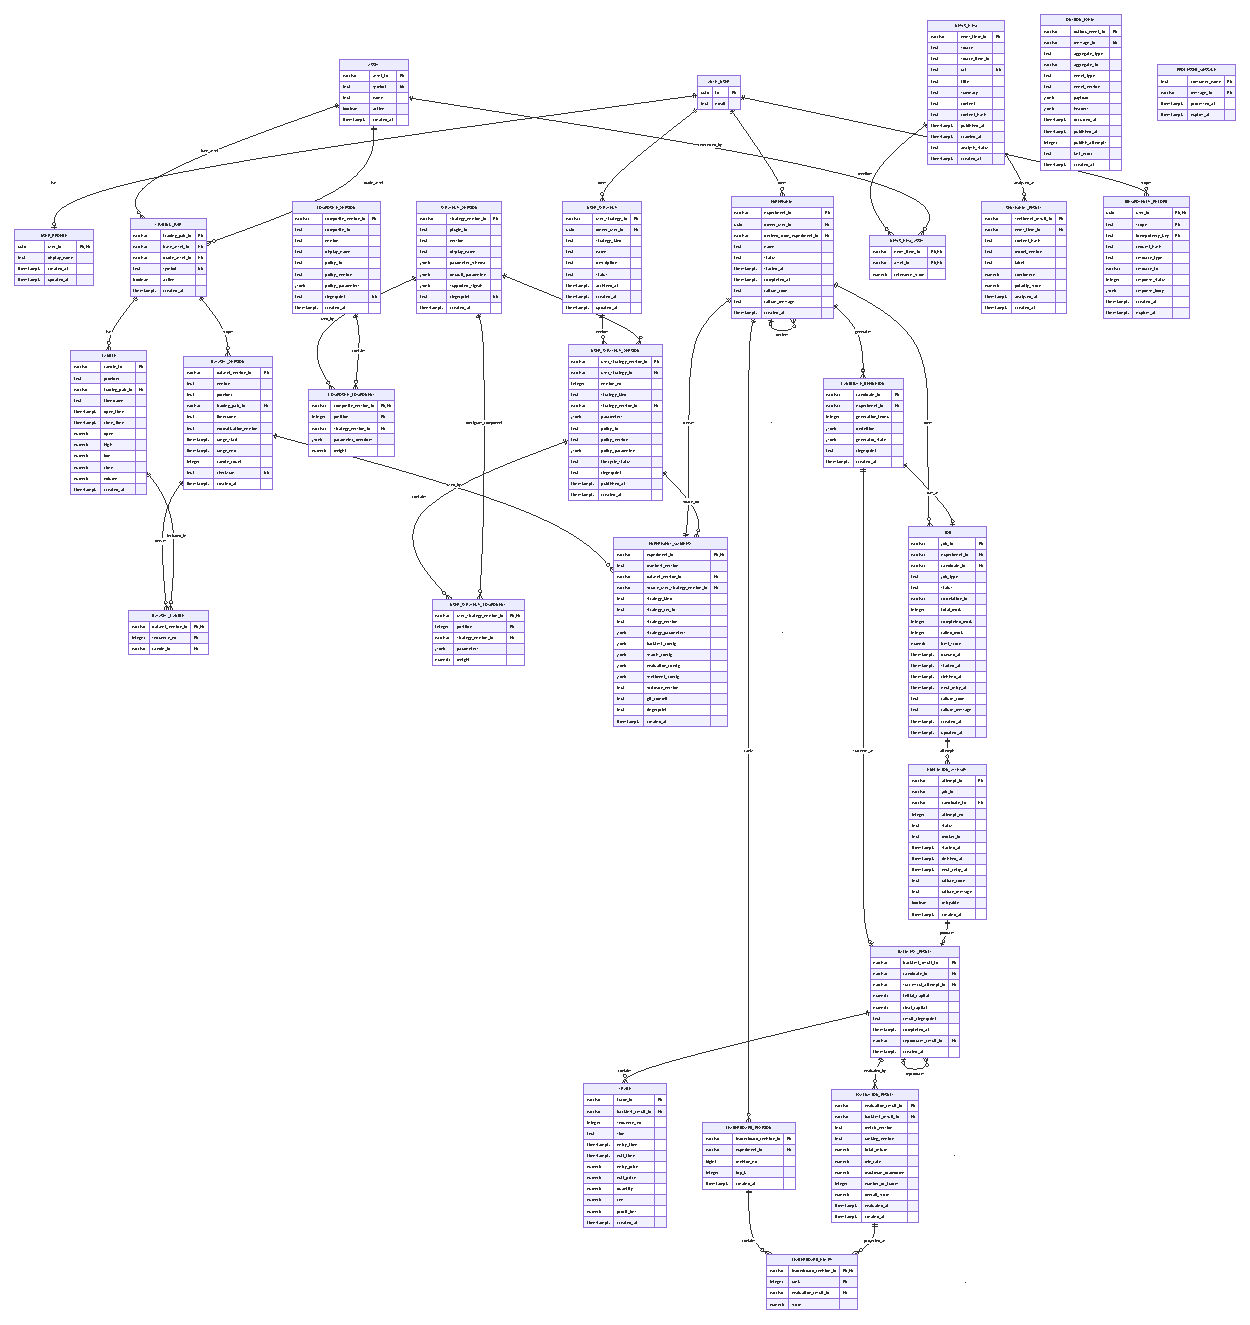
\includegraphics[width=0.99\linewidth,height=0.79\textheight,keepaspectratio]{erd-full.pdf}
  \caption{ERD đầy đủ của PostgreSQL business schema}
  \label{fig:erd-full}
  \sourceNote{\texttt{docs/database/drawio-erd.mmd}; migration trong \texttt{supabase/migrations}.}
\end{figure}

\begin{longtable}{L{3cm}L{2.8cm}L{3.7cm}L{3.5cm}}
  \caption{Event/message catalog rút gọn}\label{tab:event-catalog}\\
  \toprule
  \rowcolor{TableHeader}
  \textbf{Message/event} & \textbf{Producer} & \textbf{Consumer/ý nghĩa} & \textbf{Correctness rule} \\
  \midrule
  \endfirsthead
  \toprule
  \rowcolor{TableHeader}
  \textbf{Message/event} & \textbf{Producer} & \textbf{Consumer/ý nghĩa} & \textbf{Correctness rule} \\
  \midrule
  \endhead
  SEARCH\_REQUEST v1 & API/Execution Outbox & Search Coordinator bắt đầu/resume run. & Stable run/job identity, version fence. \\
  BACKTEST\_JOB & Search/Execution Outbox & Backtest Worker xử lý Candidate. & At-least-once; ACK sau commit; dedup Result. \\
  CANDIDATE\_EVALUATED & Worker Outbox & Ranking và Coordinator. & Hai Consumer Group độc lập; idempotent score/reconcile. \\
  PROGRESS/STATUS & Worker/Execution & API WebSocket và UI. & Chỉ là update hint; REST snapshot authoritative. \\
  LEADERBOARD\_REVISION & Ranking & API/Web cập nhật Top-K. & Revision tăng đơn điệu; client bỏ stale. \\
  NEWS\_ANALYSIS & News/Worker & Sentiment processing lifecycle. & Lease/attempt active mới được complete. \\
  DEAD\_LETTER & Worker & Operator/recovery workflow. & Redact secret; lưu reason và original identity. \\
  \bottomrule
\end{longtable}

\chapter{Bảng tự đánh giá và đóng góp thành viên}
\label{app:self-assessment}

\section{Nguyên tắc đọc bảng}

Các mức trong \cref{tab:self-score} được chép từ \texttt{File Danh Gia.xlsx} và mang nhãn \textbf{nhóm tự đánh giá}. Chúng không đồng nghĩa với trạng thái VERIFIED. Ma trận evidence ở \cref{chap:evaluation} mới là nơi phân biệt Verified, Partial, Blocked và No Claim.

\begin{longtable}{C{0.8cm}L{7.4cm}C{1.8cm}L{3cm}}
  \caption{Mức tự đánh giá của nhóm theo rubric}\label{tab:self-score}\\
  \toprule
  \rowcolor{TableHeader}
  \textbf{STT} & \textbf{Tiêu chí} & \textbf{Tự đánh giá} & \textbf{Ghi chú evidence} \\
  \midrule
  \endfirsthead
  \toprule
  \rowcolor{TableHeader}
  \textbf{STT} & \textbf{Tiêu chí} & \textbf{Tự đánh giá} & \textbf{Ghi chú evidence} \\
  \midrule
  \endhead
  1 & Khả năng mở rộng Strategy/Plugin & 4/4 & Có link code/test/ADR. \\
  2 & Tách trách nhiệm và giảm coupling & 4/4 & Có architecture tests; evidence tổng Partial. \\
  3 & Khả năng thay thế thành phần & 4/4 & Boundary có; thiếu demo thay thế LIVE. \\
  4 & Scalability và Performance & 4/4 & Có benchmark in-process. \\
  5 & Realtime và Multi-timeframe & 4/4 & Thiếu Binance LIVE evidence. \\
  6 & Reliability và Observability & 4/4 & Redis verified; full LIVE isolation còn thiếu. \\
  7 & Reproducibility và Versioning & 4/4 & Có reproduction evidence. \\
  8 & Market Data và Candlestick & 4/4 & Controlled/browser evidence. \\
  9 & Strategy Engine $\geq 4$ strategy & 4/4 & Bốn plugin được kiểm chứng. \\
  10 & Composite Strategy & 4/4 & Thiếu published LIVE version ID. \\
  11 & Backtesting Engine & 4/4 & Có code/test; LIVE DB journey còn thiếu. \\
  12 & Strategy Evaluation & 4/4 & Bốn metric có contract/test. \\
  13 & Search và Stop Condition & 4/4 & Random/bounded flow có test. \\
  14 & Leaderboard Top-K & 4/4 & Thiếu revision ID từ LIVE run. \\
  15 & Visualization Strategy và Trade & 4/4 & Prototype/controlled; thiếu ảnh LIVE. \\
  16 & News Collector & 4/4 & Provider/storage LIVE chưa hoàn tất. \\
  17 & Sentiment Analysis & 4/4 & Sheet còn ghi kế hoạch hoàn thiện integration. \\
  18 & Source code và README & 4/4 & Repository evidence đầy đủ. \\
  19 & Architecture Document & 4/4 & C4/module/data-flow đã có. \\
  20 & Architectural Decision Records & 4/4 & 17 ADR trong index. \\
  21 & Video/demo và link minh chứng & 4/4 & Video/report link còn trống trong sheet. \\
  22 & Demo end-to-end & 4/4 & Full LIVE evidence đang Blocked. \\
  23 & Scenario kiến trúc/xử lý lỗi & 4/4 & Ô evidence trong sheet chính đang trống. \\
  24 & Phần nâng cao có mục tiêu kiến trúc rõ & 4/4 & Evidence matrix chính giữ NO CLAIM. \\
  \bottomrule
\end{longtable}

\section{Đóng góp thành viên}

Sheet thành viên hiện ghi mức đóng góp bằng nhau như \cref{tab:contributions}, nhưng các cột vai trò, công việc và minh chứng chưa được điền. Báo cáo không tự suy diễn từ lịch sử commit.

\begin{table}[H]
  \centering
  \caption{Thông tin đóng góp đã có trong bảng tự đánh giá}
  \label{tab:contributions}
  \begin{tabularx}{\textwidth}{C{1cm}L{2.8cm}YL{2.5cm}Y}
    \toprule
    \rowcolor{TableHeader}
    \textbf{STT} & \textbf{MSSV} & \textbf{Họ và tên} & \textbf{Đóng góp} & \textbf{Vai trò/minh chứng} \\
    \midrule
    1 & 23127221 & Nguyễn Tiến Luật & 25\% & Chưa cập nhật trong sheet. \\
    2 & 23127228 & Phạm Văn Minh & 25\% & Chưa cập nhật trong sheet. \\
    3 & 23127281 & Đặng Nghi Văn & 25\% & Chưa cập nhật trong sheet. \\
    4 & 23127494 & Nguyễn Huỳnh Tiến & 25\% & Chưa cập nhật trong sheet. \\
    \midrule
    \multicolumn{3}{r}{\textbf{Tổng}} & \textbf{100\%} & \\
    \bottomrule
  \end{tabularx}
\end{table}

\chapter{Liên kết bàn giao và hướng dẫn tái lập}
\label{app:links}

\section{Repository}

\begin{center}
\href{https://github.com/PhamVanMinhBinhThuan/crypto-strategy-platform}{%
\textbf{https://github.com/PhamVanMinhBinhThuan/crypto-strategy-platform}}
\end{center}

Repository là nguồn chính thức của source code, migration, automated tests, architecture documentation, ADR và evidence. Khi trích evidence cần ghi commit SHA tương ứng thay vì chỉ dùng link nhánh có thể thay đổi.

\section{Hướng dẫn setup, cài đặt và build}

\begin{center}
\href{https://github.com/PhamVanMinhBinhThuan/crypto-strategy-platform/blob/main/docs/SETUP.md}{%
\textbf{GitHub — docs/SETUP.md}}
\end{center}

Hướng dẫn bao gồm prerequisites, environment variables, PostgreSQL/Supabase migration, Redis, Sentiment, API, Worker, Web, build, test, health check và troubleshooting cho Windows/macOS/Linux.

\section{Tài liệu kiến trúc liên quan}

\begin{itemize}
  \item Architecture index: \url{https://github.com/PhamVanMinhBinhThuan/crypto-strategy-platform/tree/main/docs/architecture}
  \item ADR index: \url{https://github.com/PhamVanMinhBinhThuan/crypto-strategy-platform/tree/main/docs/adr}
  \item API documentation: \url{https://github.com/PhamVanMinhBinhThuan/crypto-strategy-platform/tree/main/docs/api}
  \item Database documentation: \url{https://github.com/PhamVanMinhBinhThuan/crypto-strategy-platform/tree/main/docs/database}
  \item Demo runbook: \url{https://github.com/PhamVanMinhBinhThuan/crypto-strategy-platform/tree/main/docs/demo}
\end{itemize}

\section{Lệnh biên dịch báo cáo}

Từ thư mục \texttt{docs}, chạy XeLaTeX hai lần để cập nhật mục lục, danh mục hình/bảng và cross-reference:

\begin{verbatim}
xelatex -interaction=nonstopmode -halt-on-error main.tex
xelatex -interaction=nonstopmode -halt-on-error main.tex
\end{verbatim}

Các sơ đồ Mermaid đã được render sẵn thành PDF trong \texttt{report-assets/diagrams}; quá trình biên dịch báo cáo không cần Node.js, Mermaid CLI hoặc \texttt{shell-escape}.

\end{document}
